% !TEX TS-program = pdflatex
% !TEX encoding = UTF-8 Unicode

% This is a simple template for a LaTeX document using the "article" class.
% See "book", "report", "letter" for other types of document.

\documentclass[11pt]{article} % use larger type; default would be 10pt
\usepackage[utf8]{inputenc} % set input encoding (not needed with XeLaTeX)

%%% Examples of Article customizations
% These packages are optional, depending whether you want the features they provide.
% See the LaTeX Companion or other references for full information.

%%% PAGE DIMENSIONS
\usepackage{geometry} % to change the page dimensions
\geometry{a4paper} % or letterpaper (US) or a5paper or....
% \geometry{margin=2in} % for example, change the margins to 2 inches all round
% \geometry{landscape} % set up the page for landscape
%   read geometry.pdf for detailed page layout information

\usepackage{graphicx} % support the \includegraphics command and options

% \usepackage[parfill]{parskip} % Activate to begin paragraphs with an empty line rather than an indent

%%% PACKAGES
\usepackage{booktabs} % for much better looking tables
\usepackage{array} % for better arrays (eg matrices) in maths
\usepackage{paralist} % very flexible & customisable lists (eg. enumerate/itemize, etc.)
\usepackage{verbatim} % adds environment for commenting out blocks of text & for better verbatim
\usepackage{subfig} % make it possible to include more than one captioned figure/table in a single float
% These packages are all incorporated in the memoir class to one degree or another...

%%% HEADERS & FOOTERS
\usepackage{fancyhdr} % This should be set AFTER setting up the page geometry
\pagestyle{fancy} % options: empty , plain , fancy
\renewcommand{\headrulewidth}{0pt} % customise the layout...
\lhead{}\chead{}\rhead{}
\lfoot{}\cfoot{\thepage}\rfoot{}

%%% SECTION TITLE APPEARANCE
\usepackage{sectsty}
\allsectionsfont{\sffamily\mdseries\upshape} % (See the fntguide.pdf for font help)
% (This matches ConTeXt defaults)

%%% ToC (table of contents) APPEARANCE
\usepackage[nottoc,notlof,notlot]{tocbibind} % Put the bibliography in the ToC
\usepackage[titles,subfigure]{tocloft} % Alter the style of the Table of Contents
\renewcommand{\cftsecfont}{\rmfamily\mdseries\upshape}
\renewcommand{\cftsecpagefont}{\rmfamily\mdseries\upshape} % No bold!

%%% END Article customizations
\usepackage{xcolor}
\usepackage{tcolorbox}
\usepackage{lipsum}  % 示例文本
\usepackage{mdframed}
\usepackage{pdfpages}


% R code support
\usepackage{listings}
% \lstset{language=R,  % 设置语言为R
%         basicstyle=\ttfamily, % 设置字体样式
%         numbers=left,  % 行号显示在左侧
%         numberstyle=\small\color{blue},  % 行号样式
%         frame=single,  % 设置代码块的边框
%         backgroundcolor=\color{lightgray},  % 设置代码块的背景颜色
%         }

\usepackage{graphicx}
\usepackage{float}
\usepackage{amsmath}
% \usepackage{hyperref}
\usepackage[hidelinks]{hyperref}


% 设置R语言代码高亮
\lstdefinestyle{rstyle}{
  language=R,
  basicstyle=\ttfamily,
  numbers=left,
  numberstyle=\tiny\color{gray},
  commentstyle=\color{green!40!black},
  keywordstyle=\color{blue},
  stringstyle=\color{purple},
  morekeywords={read.csv},
  frame=single,
  breaklines=true
}

\usepackage{tabularx}
\usepackage{longtable}

% Set line spacing to 1.5
\usepackage{setspace}
\onehalfspacing
% Set up encoding and font usage
\usepackage[T1]{fontenc}
\usepackage{lmodern} % Similar to Arial, sans-serif
% 
\title{Deciphering Abalone Ages \\ through Machine Learning Methods}
\author{\textbf{Anonymous Marking Code}: Z0195806}
\begin{document}
\maketitle
% 
% 
% 
\tableofcontents
% 
% 
\section{Introduction}
\subsection{Background}
\paragraph{Traditional methods of determining the age of abalones involve cutting open the abalone shells at the cone, staining them, and then counting the rings under a microscope. This process is time-consuming and destructive, relies on manual effort, and is subject to the subjective judgement of technicians, potentially causing harm to the abalones. These factors limit the efficiency and accuracy of the method, prompting researchers to seek better solutions. Alternative, more readily obtainable measurements may be used to predict age, but might require additional information such as weather patterns, location, and food supply.}
% 
\paragraph{In this report, I leverage the UCI Abalone dataset \cite{misc_abalone_1}, which contains physical measurements of abalones (such as length, height, and total weight), and use R's tidyverse to build a machine learning model. This approach offers a more sophisticated method for predicting the age of abalones.}
% 
% 
\subsection{Data Set Introduction}
% 
\paragraph{The table (Table 1) is some description of the data set, in which Sex, Length, Diameter, Height, Whole\_weight, Shucked\_weight, Viscera\_weight and Shell\_weight are the predictor variables. The target variable Age does not appear in the data set, but its value is equal to Rings+1.5.}
% 
% 
\begin{table}[h]
    \centering
    \begin{tabular}{l l l l}
        \hline
        \textbf{Variable Name} & \textbf{Type} & \textbf{Description}        & \textbf{Units} \\ \hline
        Sex                    & Categorical   & M, F, and I (infant)        & -              \\
        Length                 & Continuous    & Longest shell measurement   & mm             \\
        Diameter               & Continuous    & Perpendicular to length     & mm             \\
        Height                 & Continuous    & With meat in shell          & mm             \\
        Whole\_weight          & Continuous    & Whole abalone               & grams          \\
        Shucked\_weight        & Continuous    & Weight of meat              & grams          \\
        Viscera\_weight        & Continuous    & Gut weight (after bleeding) & grams          \\
        Shell\_weight          & Continuous    & After being dried           & grams          \\
        Rings                  & Integer       & +1.5 gives the age in years & -              \\ \hline
    \end{tabular}
    \caption{Abalone Dataset Variable Description}
    \label{table:abalone_vars}
\end{table}
% 
% 
\subsection{Model in Use}
% 
% 
\paragraph{In the report, two types of machine learning algorithms, linear regression with Lp regularization and random forest, were used to train the processed training set. The performance of the two models was then compared based on their performance on the test set.}
% 
% 
\begin{figure}[h]
    \centering
    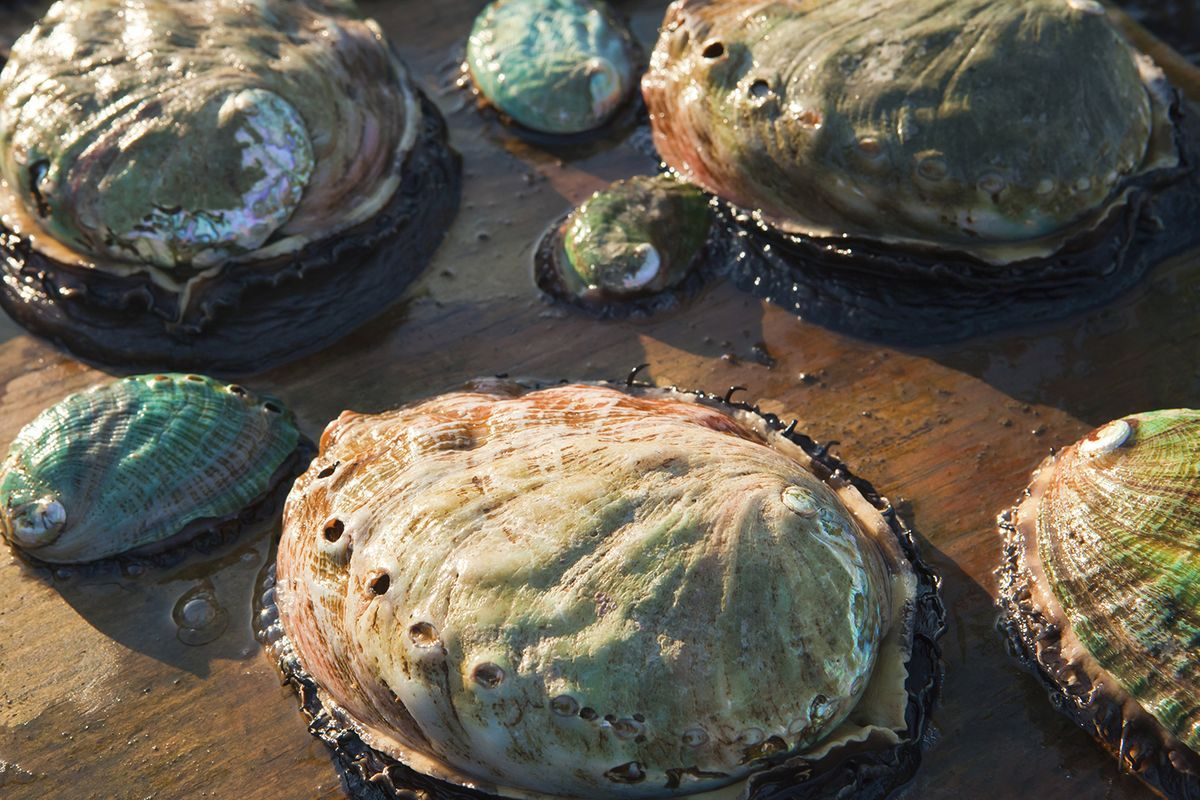
\includegraphics[width=0.5\textwidth]{Pic/Abalone.jpg}
    \caption{Pic of Abalone}
\end{figure}
% 
% 
\section{Data Pre-processing and EDA}
\paragraph{\textbf{Details on the datasets used in Parts 2, 3, and 4 can be found in the Appendix.}}
\subsection{Data Pre-processing}
\subsubsection{Data Cleaning}
\paragraph{Since all columns in the dataset, except for the Sex column, contain continuous data, there were no typographical errors found upon inspection. Also, using \textbf{any(is.na(dataset))} revealed no missing values in the data.}
\paragraph{Before executing machine learning tasks, it's crucial to inspect the dataset, as ambiguous data in the training set can lead to biases in model training. At the same time, I identified some logical inconsistencies in the data and used the filter from tidyverse to remove these rows from the dataset:}
\begin{enumerate}
    \item There were 2 instances where the Height was equal to 0, which is impossible for abalones;
    \item Theoretically, the total weight of an abalone should equal the sum of its parts, but there were a significant number of rows (15 rows) where: $$WholeWeight < ShuckedWeight + ShellWeight$$
\end{enumerate}
\subsubsection{Add Age Column}
\paragraph{Although using "Rings" might be slightly simpler and keep the prediction task closer to the original data structure, using "Age" can make the prediction more interpretable from a biological perspective, as it directly represents the age of the abalones. Hence, I added a new column named Age using the formula Age = Rings + 1.5 and removed the original Rings column.}
\subsubsection{Dealing with Sex Columns}
\paragraph{Machine learning algorithms typically require numerical input, and the "Sex" column in the Abalone dataset contains categorical values "F" (female), "M" (male), and "I" (infant), which need to be encoded before they can be effectively used in most machine learning models.}
\paragraph{One-hot encoding converts each category value into a new binary column and assigns a 1 or 0 (True/False) value to those columns. For the 'Sex' column with three categories, it would create three new columns, one for each category ('F', 'M', 'I'), with binary values indicating the presence of each category. Here, I added three new columns named SexM, SexF, SexI, and deleted the Sex column.}
% 
% 
\subsection{Exploratory Data Analysis}
\subsubsection{Descriptive Statistics for Single Variables}
\paragraph{Descriptive statistics for a single variable involve summarizing and analyzing data to describe the main characteristics of the abalone dataset without making any assumptions about the data generation process. In this section, using the original dataset (abalone\_origin), measures of central tendency (such as mean and median), measures of variability (such as range, variance, and standard deviation, Figure 2), and graphical representations (such as histograms, Figure 3) were analyzed.}
% 
% 
% 
\begin{figure}[H]
    \centering
    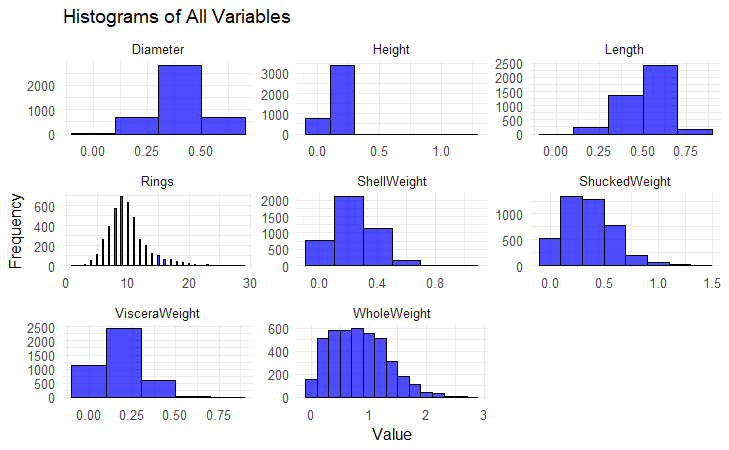
\includegraphics[width=0.9\textwidth]{Pic/Hist.png}
    \caption{Histograms of Variables}
\end{figure}
% 
% 
% 
\begin{figure}[H]
    \centering
    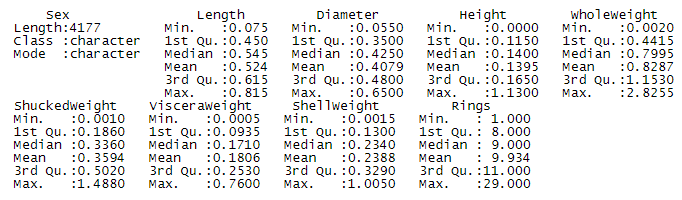
\includegraphics[width=0.9\textwidth]{Pic/discripstat.png}
    \caption{Descriptive Statistical Data}
\end{figure}
% 
% 
\subsubsection{Analysis of Correlations Between Variables}
\paragraph{Bivariate analysis can clearly show how each feature is influenced by the presence of other features. It also helps us understand and identify significant features, overcome multicollinearity effects and interdependencies, thus providing insights into hidden noise patterns in the data.}
\paragraph{In this section, using the abalone\_Age\_DummySex dataset, we were particularly interested in the impact of gender factors on age prediction. The correlation analysis charts showed that the relationships between the three genders and other variables are two parallel lines, suggesting that gender has no correlation with other predictors or age. This can be a reference for subsequent modeling. However, correlation analysis is just a basic method and not sufficient to support the removal of the Sex variable (Figure 4).}
% 
% 
\begin{figure}[H]
    \centering
    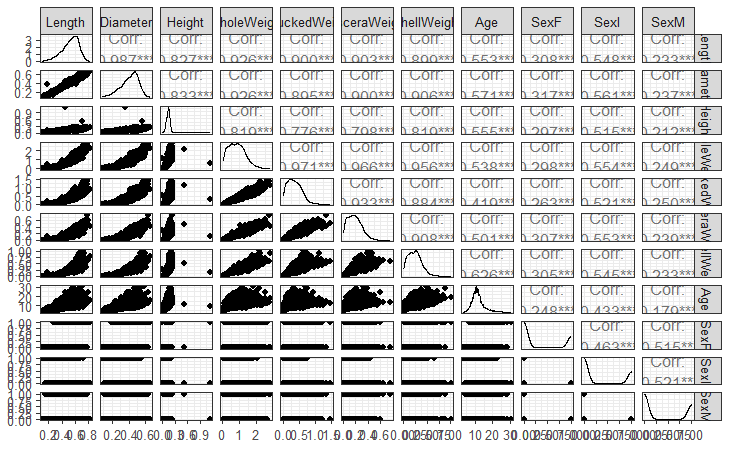
\includegraphics[width=0.75\textwidth]{Pic/ggpairs.png}
    \caption{Correlation Plot between Variables}
\end{figure}
% 
% 
% 
\subsubsection{Best Subset Selection}
\paragraph{With multiple features in the abalone dataset, directly using all predictors as model inputs is not a wise choice; it's necessary to filter input variables. Since the number of variables in the abalone dataset is not large, we opted for best subset selection here. In statistics and machine learning, best subset selection is a method used to select the best subset of predictors from a set of predictors to build a model.}
\paragraph{I applied the regsubsets function from the leaps package to both the abalone\_Age\_DummySex and abalone\_Age\_NoSex datasets to find the best subset for each. The following conclusions were drawn: 1. On the abalone\_Age\_DummySex dataset with Dummy variables, the function returned "1 linear dependencies found Warning," indicating that the dataset contains linearly dependent variables, which is not favorable for regression prediction. 2. On the dataset without Sex, the best subset contained 6 variables (7 in total, Figure 5) and did not include Height, showing consistency in the Adj Rsq, BIC, Cp charts. These conclusions provide statistical support for later modeling but do not result in the deletion of any variables.
}
% 
% 
\begin{figure}[H]
    \centering
    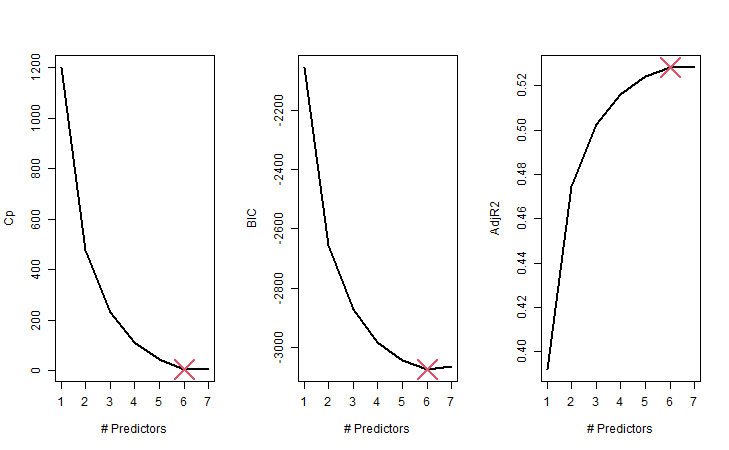
\includegraphics[width=0.8\textwidth]{Pic/BSS.png}
    \caption{Best Subset Selection}
\end{figure}
% 
% 
\section{Modeling}
\paragraph{In the machine learning modeling section of the report, Lp Norm linear regression and random forest algorithms were employed. The core methodology of this section is divided into two steps: 1. Splitting the dataset into a training set and a testing set (approximately at an 8:2 ratio), using a fixed random seed to ensure consistent results across multiple trainings and tests; 2. Encapsulating the process of training the machine learning model on the training set, making predictions on the test set, calculating model error using RMSE, and visualization into a pipeline (by calling perform\_cv\_glmnet and perform\_random\_forest) to swiftly execute the machine learning workflow on the dataset.
}
\begin{figure}[H]
    \centering
    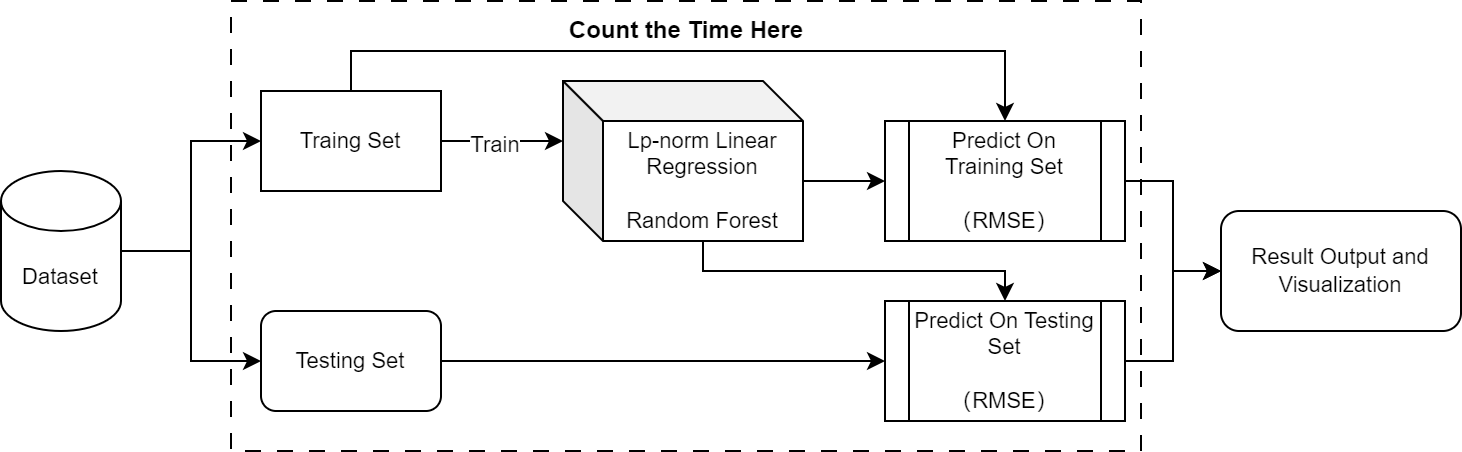
\includegraphics[width=\textwidth]{Pic/Pipeline.png}
    \caption{Machine Learning Pipeline}
\end{figure}
\paragraph{Dataset configurations: abalone\_Age, abalone\_Age\_Dummysex, abalone\_age\_NoSex, SexM, SexF, SexI, and their corresponding training and testing sets split for each dataset. These datasets meet a variety of analytical needs.}
% 
\subsection{Lp Norm Linear Regression (Ridge, LASSO, and Elastic Net)}
\subsubsection{Reason for choosing this instead of Decision Tree}
\paragraph{Linear regression models, including those with regularization, are generally more interpretable than decision tree models. In Lasso, Ridge, and Elastic Net regressions, the weight of each feature can be directly interpreted as its impact on the target variable, which is crucial for statistical analysis and result interpretation. Lasso regression (L1 regularization) is particularly suited for feature selection as it can shrink the coefficients of unimportant features to zero. If there are many unimportant features in the abalone dataset, Lasso regression can automatically perform feature selection and simplify the model. Ridge regression (L2 regularization) is particularly useful if the features in the abalone dataset are highly correlated (multicollinearity). Ridge regression reduces the variance of parameter estimates by adding a regularization term, thereby improving the model's stability and generalization ability.}
\subsubsection{Introduction to Lp Norm Linear Regression}
\paragraph{Lp linear regression is a set of methods that optimize the model by introducing regularization terms to the traditional linear regression. These regularization techniques aim to address issues like overfitting, multicollinearity, and, in some cases, perform feature selection.}
% 
% 
\subsubsection{Introduction to Lp Norm Linear Regression}
\paragraph{Lp linear regression is a set of methods that optimize the model by introducing regularization terms to the traditional linear regression. These regularization techniques aim to address issues like overfitting, multicollinearity, and, in some cases, perform feature selection.}
\subsubsection{Model Assumption}
\begin{enumerate}
    \item Linearity assumption: The model assumes a linear relationship between the predictor variables (such as the abalone's length, diameter, height, weight, etc.) and the response variable (such as age or rings). This means the response variable can be expressed as a weighted sum of the predictor variables plus an error term.
    \item Multicollinearity assumption: While traditional linear regression models assume no perfect multicollinearity among predictor variables, Lp linear regression can tolerate a certain degree of multicollinearity and mitigate its adverse effects through regularization. If the predictor variables in the abalone dataset are highly correlated (like whole weight and shucked weight), using Ridge or Elastic Net might be more appropriate as these methods can handle such multicollinearity.
    \item Proper choice of alpha and lambda: The model assumes that the alpha and lambda values chosen through cross-validation produce a well-regularized model that is neither overfit nor underfit.
    \item Proper representation of the feature space: The model assumes that the input features have been properly transformed or selected to allow the linear model to capture the relationships between the target variable and the features.
\end{enumerate}
% 
% 
\subsubsection{Design of Experiment (DoE)}
\paragraph{As mentioned at the beginning of part 3, five datasets were set up to meet various analytical needs, and I set three different alpha values (0, 0.5, 1), corresponding to Ridge, Elastic Net, and Lasso regression, theoretically requiring 15 machine learning analyses to analyze results. Due to time constraints and the energy required to analyze 15 outcomes, I designed the following experimental methods for analysis: The first part uses the same dataset with different alpha values to verify model assumption three; the second part uses different datasets with the same alpha value to verify model assumption four. This allows conclusions to be drawn from 8 experiments. The experimental design is as follows:}
\begin{figure}[H]
    \centering
    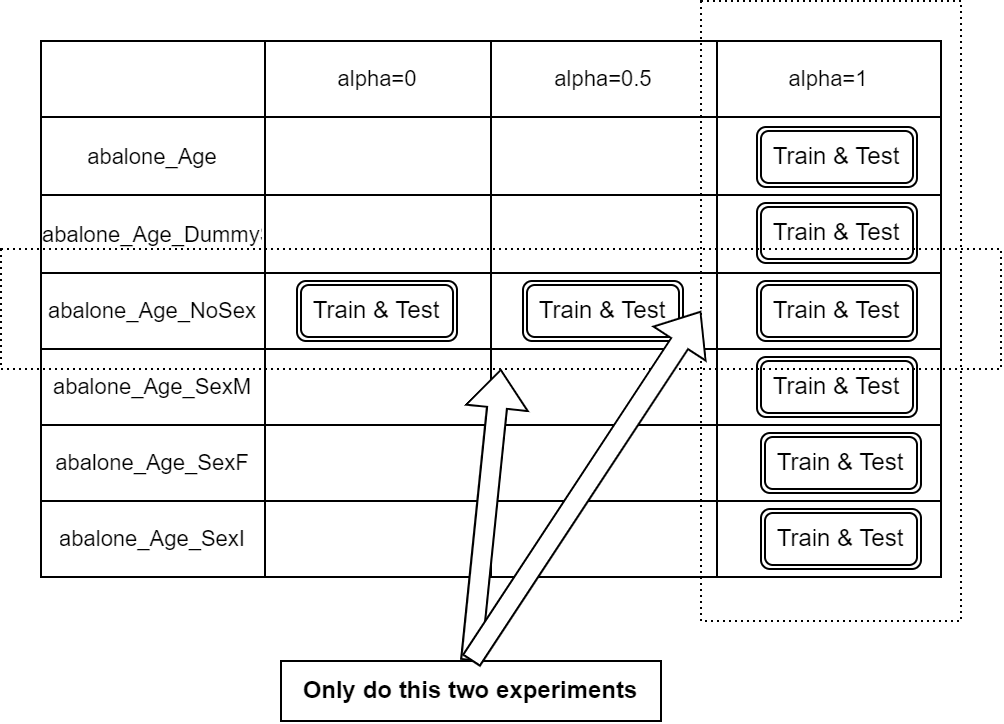
\includegraphics[width=0.8\textwidth]{Pic/DoE.png}
    \caption{Design of Experiment}
\end{figure}
% 
\subsubsection{Result Analysis}
\paragraph{Since model assumptions 1 and 2 have been proven correct in part 2, I will focus on analyzing based on assumptions 3 and 4. According to the experimental results, it was found:}
\begin{enumerate}
    \item On the same dataset \texttt{Abalone\_Age\_NoSex}, by changing the value of $\alpha$, the model's final error RMSE on both the training and testing sets was between 2.1 and 2.2, changing as $\alpha$ changed from 0 to 1, but not significantly.
    \item After dividing the data into three groups by sex, the RMSE of the Infant dataset was much lower than that of the \texttt{Abalone\_Age\_NoSex} dataset, while the RMSEs of the SexM and SexF datasets were slightly higher than that dataset, showing a significant change in model performance, which may reflect the inherent differences in samples of different genders. This means that if the prediction effect on SexI is better after splitting.
    \item In the second part of the experiment, with $\alpha=1$, as lambda increases, the best model has only 6 variables, and the variable with a coefficient of 0 is Height. This is the same as the result of the Best Subset Selection in Part 2. At the same time, the optimal $\lambda_{\text{min}}$ values of different datasets are different, indicating that different characteristics of the data may require different degrees of regularization.
    \item Model performance: Looking at the RMSE, Ridge regression ($\alpha=0$) performed best on this specific dataset, although the improvement was very minimal. The performance of the elastic network ($\alpha=0.5$) and LASSO regression ($\alpha=1$) was similar but slightly inferior.
    \item Variable selection: LASSO regression performs variable selection by reducing some coefficients to zero, while the elastic network and Ridge regression retain all variables. This may mean that LASSO or an elastic network (when alpha is close to 1) might be more applicable when variable selection is needed.
    \item Regularization strength: The value of $\lambda_{\text{min}}$ decreases as alpha decreases, indicating that stronger regularization may be needed for Ridge regression to achieve optimal performance.
\end{enumerate}
% 
% 
\begin{figure}[H]
    \centering
    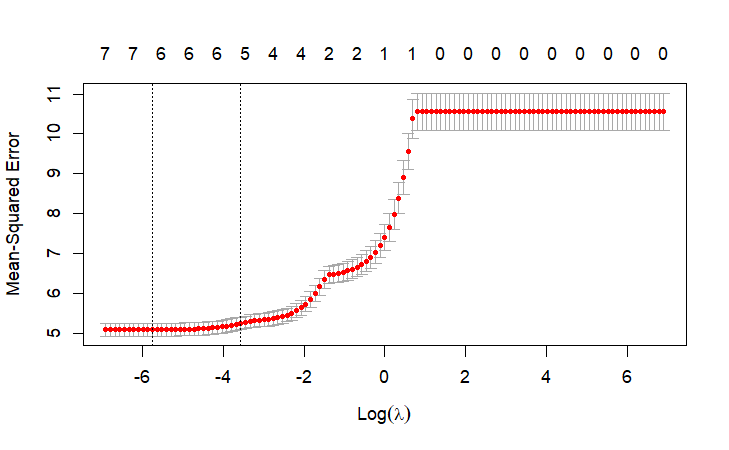
\includegraphics[width=0.8\textwidth]{Pic/lasso.png}
    \caption{Lasso Regression with abalone\_Age\_NoSex Dataset}
\end{figure}
% 
\begin{figure}[H]
    \centering
    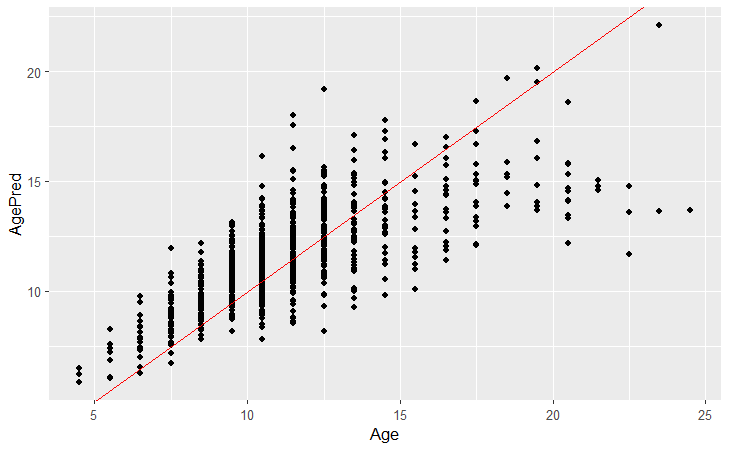
\includegraphics[width=0.8\textwidth]{Pic/lasso_performance.png}
    \caption{The Pridicted Value vs True}
\end{figure}
% 
% 
% 
\subsection{Random Forest}
\subsubsection{Reason for choosing This instead of Neural Network}
\paragraph{Since random forest is an ensemble method based on decision trees, it provides better model interpretability. We can easily see which features have the greatest impact on the prediction results and even interpret the decision paths of individual decision trees. In contrast, neural networks are often seen as "black box" models, difficult to interpret their internal workings and decision-making processes. Besides, unlike neural networks, it is not sensitive to the scaling of input features. Decision trees split based on the threshold of features, so there is no need for feature standardization or normalization. Due to the averaging of predictions from multiple decision trees, random forests are usually more robust to noise and outliers in the data.}
\subsubsection{Introduction to Random Forest}
\paragraph{Random forest is a popular and powerful machine learning algorithm that belongs to the category of ensemble learning methods. It consists of multiple decision trees and makes predictions by aggregating the results of these trees, thereby improving the accuracy and robustness of the model.}
\subsubsection{Model Assumption}
\begin{enumerate}
    \item Variable correlation: Random forest reduces the impact of high correlation among variables by choosing the best feature from a random subset of features at each decision tree split. Therefore, the model assumes that even if there is a certain degree of correlation among features, it will not significantly negatively affect model performance.
    \item Model complexity and overfitting: Random forest improves predictive accuracy by integrating multiple decision trees and reduces the risk of overfitting by introducing randomness. Therefore, the model assumes that it can maintain good generalization ability even on high-dimensional data or complex data structures.
    \item Feature importance: Random forest can assess the contribution of each feature to the prediction results, so the model assumes that some features may be more important than others for predicting age.
    \item No need for feature scaling: Random forest is not sensitive to the scale of features, so the model assumes that there is no need to standardize or normalize features.
\end{enumerate}
% 
\subsubsection{Model Tuning}
% 
\paragraph{When optimizing model performance using the randomForest function in R, key parameter adjustments include ntree (number of trees), mtry (number of features to consider at each split), nodesize (minimum number of samples in terminal nodes), sampsize (sample size for each tree), and maxnodes (maximum number of nodes per tree). Increasing ntree can enhance model stability, adjusting mtry affects model diversity and flexibility, and adjusting nodesize and maxnodes help prevent overfitting.}
\paragraph{In addition to the parameter adjustment within randomForest, we can also try different feature combinations multiple times when predicting Age, such as removing Sex or Height, and viewing the variance explanatory and RMSE changes of the model.}
% 
% 
% 
\subsubsection{Result Analysis}
\paragraph{In this part, I trained the random forest using four data models. The first model: using all features; the second model: excluding gender features; the third model: excluding height features; the fourth model: excluding both gender and height features. In all four models, I defaulted to using 500 trees and considering 2 variables at each split, and came to the following conclusions:}
\begin{enumerate}
    \item The impact of features: Excluding specific features (such as gender or height) has a relatively limited impact on the overall performance of the model. This may indicate that these features are not decisive factors for predicting age, or their information may have been indirectly captured by the model through other features.
    \item Training and testing errors: In all models, the training error is consistently significantly lower than the testing error. This is a typical sign of overfitting, indicating that the model may be too sensitive to the training data, capturing some noise in the training data that does not commonly exist in the testing data.
    \item Model-explained variance: All models can explain about 55\% of the variance, indicating that the random forest model has some ability to capture the intrinsic structure of the dataset, but there is still a certain proportion of variance not explained by the model, which may be caused by random noise in the data or unobserved variables.
    \item Mean squared residuals: The difference in mean squared residuals between the models is not significant, further confirming that removing a single feature has a limited impact on model predictive performance.
    \item Running time: The running time of the models is relatively consistent, indicating that the removal of features has little impact on computational efficiency. This may be because the random forest algorithm itself is highly efficient in handling features, and the number of trees in the model (500 trees) is the main factor determining the running time.
\end{enumerate}
% 
% 
\section{Model Comparison}
% 
% 
\paragraph{This table (Table 2) provides a clear comparison of key metrics between Lp linear regression and random forest.}
% 
\begin{table}[H]
    \centering
    \caption{Summary of Lp Linear Regression and Random Forest Results}
    \begin{tabular}{l c c}
        \hline
        \textbf{Metric/Model}            & \textbf{Lp Linear Regression} & \textbf{Random Forest}           \\ \hline
        Model Coefficients               & Provided for each feature     & -                                \\
        Training Error (RMSE)            & 1.55983 to 2.541056           & 1.012617 to 1.026651             \\
        Testing Error (RMSE)             & 1.646548 to 2.502254          & 2.064943 to 2.08656              \\
        Running Time                     & 0.08 to 0.14 seconds          & 4.35 to 4.51 seconds             \\
        Model Details                    & $\alpha=0,0.5,1$              & 500 trees, 2 variables per split \\
        Mean Squared Residuals           & -                             & 4.717192 to 4.764544             \\
        Percentage of Explained Variance & -                             & 54.83\% to 55.27\%               \\ \hline
    \end{tabular}
    \label{table:results_summary}
\end{table}
% 
% 
\paragraph{\textbf{Performance}: The testing errors of random forest and Ridge regression are similar, indicating that both methods have similar predictive capabilities on this specific dataset. However, random forest has a slight advantage in explaining variance.}
\paragraph{\textbf{Interpretability}: Lp-norm regression provides coefficients for features, offering better model interpretability. Although random forest can assess feature importance, its overall interpretability is not as good as linear models.}
\paragraph{\textbf{Computational efficiency}: The running time of Lp norm linear regression is much lower than that of random forest on my personal computer, especially important when dealing with large datasets. Although the ablone dataset is not big enough, I can still obeserve that difference in speed.}
\paragraph{\textbf{Handling non-linear relationships}: Random forest is better at handling non-linear relationships, while Ridge regression may need additional feature engineering to capture these relationships.
}
\paragraph{In conclusion, which model to choose depends on the specific application scenario. If model interpretability is a key consideration and the data relationships are close to linear, Lp-norm regression might be a better choice. For datasets with complex non-linear relationships or when model performance is the sole focus, random forest might offer better results, albeit at the cost of longer training time.}
% 
% 
% 
% 
\section{Results and Conclusion}
% 
% 
% 
\subsection{Conclusion}
\paragraph{The analysis of the abalone dataset through Lp linear regression and random forest models has provided valuable insights into predicting the age of abalones based on their physical measurements. The Lp linear regression, particularly Ridge regression, offered interpretable coefficients for each feature, highlighting the importance of feature selection and regularization in addressing multicollinearity and overfitting.}
\paragraph{Random forest, on the other hand, showcased its strength in handling non-linear relationships and providing robust predictions despite its longer computation time. The ability to assess feature importance in random forest models is beneficial for understanding the driving factors behind abalone age, even if the model itself is less interpretable than linear regression models.}
% 
% 
% 
\subsection{Future Work}
\paragraph{\textbf{Data Collection}: Expanding the dataset to include additional relevant features, such as environmental conditions (water temperature, salinity, etc.), could provide a more holistic view of the factors influencing abalone age. Collecting data over a longer period could also help in understanding temporal variations in growth patterns. We can even use the Embedded Equipments with sensors or camera to get more of this kind of data automatically.}
\paragraph{\textbf{Modelling Approaches}: Exploring more complex models like ensemble methods beyond random forest deep learning approaches could uncover non-linear relationships not captured by the current models. I made the tradeoff between deep learning and random forest because I was afraid about I can't explain the principle why neural network perform better when I change some parameters. Additionally, incorporating cross-validation and hyperparameter tuning more extensively could improve model performance and reliability.}
% 
% 
% 
% 
% 
% 
% 
% 
% 
% 
\bibliographystyle{unsrt}
\bibliography{References}
% 
% 
\appendix
\section{Dataset Router}
\begin{figure}[H]
    \centering
    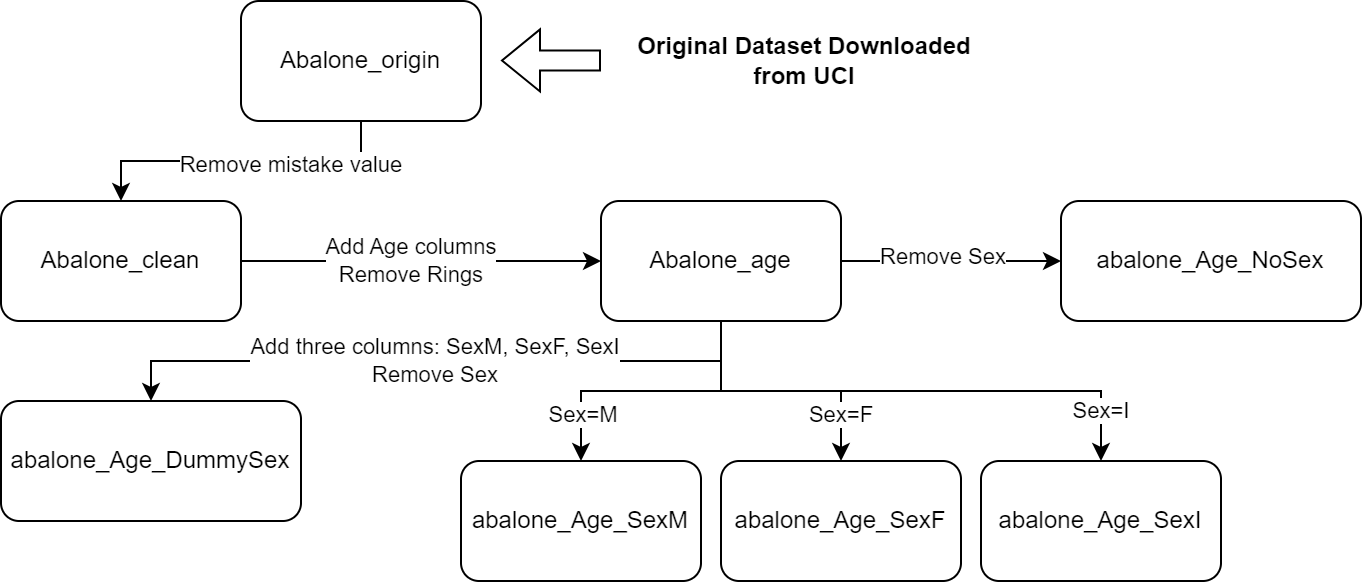
\includegraphics[width=\textwidth]{Pic/DatasetDep.png}
    \caption{Dataset Family Used in This Report}
\end{figure}
% 
% 
\section{RMarkdown Source}
\paragraph{I used rmarkwon to write and run R code analysis and output PDF version below.}
\includepdf[pages=-]{Pages/Abalone-Learning}
% 
% 
% 
% 
\end{document}
